\documentclass[letterpaper,12pt,peerreviewca,draftcls]{IEEEtran}
\usepackage{csm16,graphicx,url}

\title{Sample.tex for the CSM Style File csm.sty\\
A convenient template for typesetting\\
articles for IEEE CSM }
\author{Kent H. Lundberg \\
contact: klund@alum.mit.edu, fax 123-456-7890 \\
CSM-05-000 v1.22 --- \today}

\begin{document}
\maketitle
\CSMsetup

Modeling of large-scale stochastic phenomena with both spatial and temporal (spatiotemporal) evolution is a fundamental problem in the applied sciences.
\section{Introduction}

The IEEE Control Systems Magazine is not a journal in the usual sense.
In fact, one of the primary goals of the {\it Magazine} is to make
developments in control technology accessible to the widest possible
audience.  Therefore, the standards for quality and style of exposition
are more stringent than most journals.


When you prepare your paper for submission, you must carefully read and
follow the IEEE CSM Author's Guide \cite{CSMguide}.  You can download
the latest version of this document from the IEEE CSM web page.  The
Author's Guide is updated periodically.


In addition, we suggest that you use the LATEX document you are reading
to ensure that your submitted paper meets the specifications outlined in
the Author's Guide for typesetting.


\subsubsection{Line Spacing}


When you use the IEEE CSM template, you find that the line spacings are
set to be double spaced with an extra blank line between paragraphs.
This spacing helps the editors to read and copyedit your paper.


The page limit for IEEE CSM submission is 30 pages of text.  However,
longer survey and tutorial papers may be considered.  Please contact the
Editor-in-Chief for more information.


\section{LATEX Template}


The csm.sty style file depends on the IEEE Transactions Class file,
IEEEtran.cls by Michael Shell \cite{IEEEtran}.  A copy can be found on
CTAN \cite{ctan}.  The latest version, as of this document, is version
V1.6b.

Use the csm.sty \cite{csm.sty} package file to fix up a few formatting
issues.  After you ``begin the document'' and ``make the title'', use
the CSMsetup command to finish fixing the page style.







\section{Figure Caption Style}


IEEE CSM has a mandatory uniform style for every figure and table
caption.  This style is intended to enhance the quality and
appearance of articles. Please read these instructions carefully
to facilitate the publication of your article.

Please invest care and effort in producing interesting and
informative figure captions.  These captions can greatly enhance
your paper and the overall quality of IEEE CSM.



You may put all of your figures and tables at the end of your
paper if you wish.  If your paper is accepted, IEEE determines the
correct placement of each figure and table.


\begin{figure}[t]
\centering
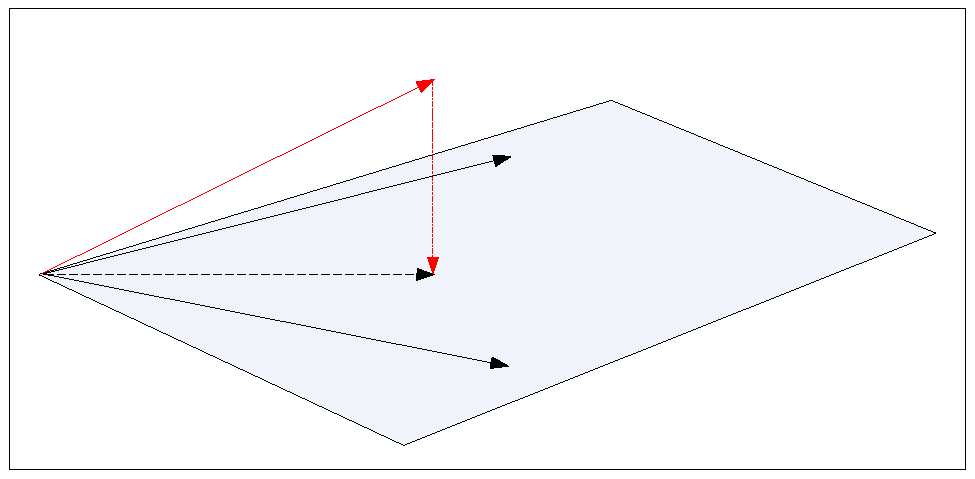
\includegraphics[scale=0.5]{sensitivity}
\caption{Title of the plot, not a sentence.  Next, a sentence is
given
  here to indicate the points that the figure is meant to
  highlight. Finally, you can include additional sentences to provide
  more detail about the meaning and importance of the figure.  These
  sentences can greatly enhance the appeal of your article.}
\label{fig1}
\end{figure}




Please note that Figure~\ref{fig1} does not have a caption or
label along the top.  The axes are labeled, and a legend is
allowed if needed. Multiple curves can be distinguished by color
or dashes and dots. The caption below the figure includes a title
and one or more sentences of pertinent information.
Figure~\ref{fig2} is an illustrative example in the proper style.



\begin{figure}[t]
\centering
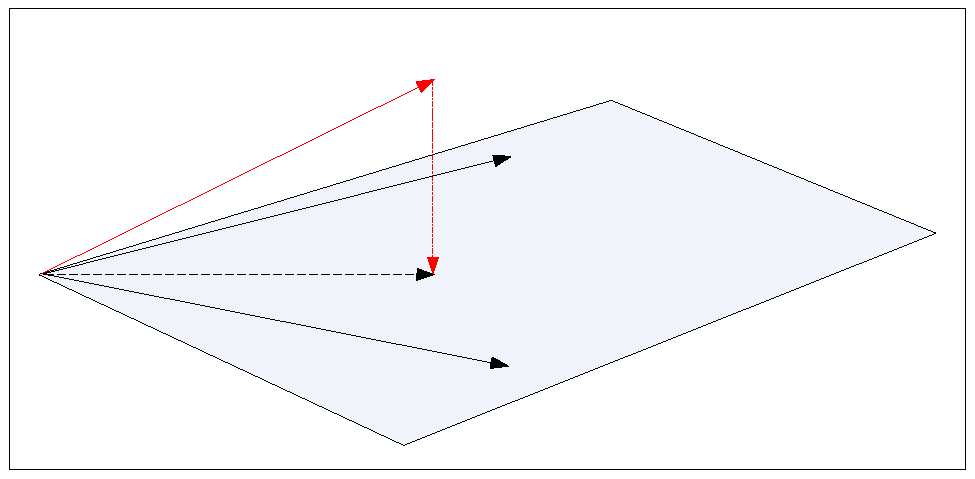
\includegraphics[scale=0.5]{sensitivity}
\caption{Bode plot of the sensitivity function.  The negative and
  positive portions of the curve suggest that the benefits of feedback
  are accompanied by a cost of feedback.  Analytical results show that
  these tradeoffs are inevitable for linear time-invariant systems whose
  relative degree is at least 2.  Analogous results for multivariable
  and time-delay systems have been developed, but are not so well
  known.}
\label{fig2}
\end{figure}














\section{Section Heading, Level A}


The style file automatically provides the correct style for
section, subsection, subsubsection, and subsubsubsection headings.
Four levels of headings can be used.  Note that the level A
heading is bold and not italic with all caps.


\subsection{Subsection Heading, Level B}


The level B heading is bold and not italic with initial caps.


\subsubsection{Subsubsection Heading, Level C}


The level C heading is bold and italic with initial caps.


\paragraph{Subsubsubsection Heading, Level D}


The level D heading is not bold and italic with initial caps.






\section{Conclusion}


We hope that these files are useful to you in preparing your submission
for IEEE CSM.  We again remind you to carefully study the IEEE CSM
Author's Guide.  If you have any questions, do not hesitate to contact
the Editor-in-Chief Dennis S. Bernstein at dsbaero@umich.edu.



\newpage

\clearpage
\bibliographystyle{unsrt}
\begin{thebibliography}{1}

\bibitem{CSMguide}
D.S. Bernstein. ``CSM Author Guide.'' Available online:
\url{http://www.ieeecss.org/PAB/csm/files/CSMAuthorGuide.pdf}


\bibitem{IEEEtran}
M. Shell.  ``IEEE Transactions class file.''  Available online:
\url{http://www.ctan.org/tex-archive/macros/latex/contrib/IEEEtran/}


\bibitem{ctan}
``The Comprehensive \TeX\ Archive Network.''
Available online: \url{http://www.ctan.org/}


\bibitem{csm.sty}
K.H. Lundberg.  ``LaTeX Style File for IEEE Control Systems Magazine.''
Available online: \url{http://www.mit.edu/klund/www/csm/}

\end{thebibliography}


\section{Author's Bio}

\noindent {\bf Kent H. Lundberg} is the Associate Editor for History of
IEEE Control Systems Magazine.  He consults for several industry
corporations and organizations and collects old textbooks on analog
computing, radar, nuclear energy, and control.

\end{document}
